\begin{enumerate}[label=\thesection.\arabic*,ref=\thesection.\theenumi]
\item A charged particle oscillates about its mean equilibrium position with a frequency of $10^9Hz$. What is the frequency of the electromagnetic waves produced by the oscillator?\\
\solution

\iffalse
\documentclass[journal,12pt,twocolumn]{IEEEtran}
\usepackage{cite}
\usepackage{amsmath,amssymb,amsfonts,amsthm}
\usepackage{algorithmic}
\usepackage{graphicx}
\usepackage{textcomp}
\usepackage{xcolor}
\usepackage{txfonts}
\usepackage{listings}
\usepackage{enumitem}
\usepackage{mathtools}
\usepackage{float}
\usepackage{gensymb}
\usepackage{comment}
\usepackage[breaklinks=true]{hyperref}
\usepackage{tkz-euclide} 
\usepackage{listings}
\usepackage{gvv}                                        
\def\inputGnumericTable{}                                 
\usepackage[latin1]{inputenc}                                
\usepackage{color}                                            
\usepackage{array}                                            
\usepackage{longtable}                                       
\usepackage{calc}                                             
\usepackage{multirow}                                         
\usepackage{hhline}                                           
\usepackage{ifthen}                                           
\usepackage{lscape}
\usepackage{amsmath}
\newtheorem{theorem}{Theorem}[section]
\newtheorem{problem}{Problem}
\newtheorem{proposition}{Proposition}[section]
\newtheorem{lemma}{Lemma}[section]
\newtheorem{corollary}[theorem]{Corollary}
\newtheorem{example}{Example}[section]
\newtheorem{definition}[problem]{Definition}
\newcommand{\BEQA}{\begin{eqnarray}}
\newcommand{\EEQA}{\end{eqnarray}}
\newcommand{\define}{\stackrel{\triangle}{=}}
\theoremstyle{remark}
\newtheorem{rem}{Remark}

\begin{document}

\bibliographystyle{IEEEtran}
\vspace{3cm}

\title{NCERT Discrete - 11.9.1.8}
\author{EE23BTECH11045 - Palavelli Srija$^{*}$}

\maketitle
\newpage
\bigskip

\renewcommand{\thefigure}{\theenumi}
\renewcommand{\thetable}{\theenumi}

\vspace{3cm}
\textbf{Question 11.9.1.8:} 
\begin{enumerate}
\item Find the seventh term of the sequence where the nth term is given by $a_n= \frac {n^2}{2^{n}}$
\end{enumerate}

\textbf{Solution: }
\fi
\begin{align}
 x(n) &= \frac{(n+1)^2}{2^{(n+1)}}u(n)
\end{align}

\begin{table}[h!]
    \centering
     \begin{tabular}{|c|c|}
        \hline
        \textbf{Parameter} & \textbf{Value} \\
        \hline
        \(x(n)\) & \(\frac{(n+1)^2}{2^(n+1)}u(n)\) \\ \\
        \(x(6)\) & ? \\
        \hline
    \end{tabular}

    \caption{Input Parameters}
    \label{tab:table_9.8.1}
\end{table}

\begin{align}
x(6) &= \frac{(6+1)^2}{2^{(6+1)}}\\
     &= \frac {49}{128}
\end{align}

\begin{enumerate}
   \item Scaling property:
     \begin{align}
         a^{n} u(n) & \xleftrightarrow{\mathcal{Z}}  \frac{1}{(1-az^{-1})}, \quad \lvert z \rvert > \lvert a \rvert 
     \end{align}
     
   \item Differentiation property:
    \begin{align}
     n u(n) & \xleftrightarrow{\mathcal{Z}} (-z) \frac{dY(z)}{dz} \\
     \implies n u(n) & \xleftrightarrow{\mathcal{Z}}  \frac{z^{-1}}{(1-z^{-1})^2}, \quad \lvert z \rvert > 1 \\
     \implies n^2 u(n) & \xleftrightarrow{\mathcal{Z}}  \frac{z^{-1}(1+z^{-1})}{(1-z^{-1})^3}, \quad \lvert z \rvert > 1
   \end{align}
   
   \item Time shifting property:
    \begin{align}
         y(n-k) & \xleftrightarrow{\mathcal{Z}} z^{-k}Y(z)
     \end{align}
\end{enumerate}

The Z transform of $x(n)$ is given by:\\
from(4)
\begin{align}
\frac{u(n)}{2^n} & \xleftrightarrow{\mathcal{Z}}  \frac{1}{(1-(2z)^{-1})}, \quad \lvert z \rvert>\frac{1}{2}
\end{align}
	from(5)
\begin{align}
\frac{n}{2^n} u(n) & \xleftrightarrow{\mathcal{Z}} \frac{(2z)^{-1}}{(1-(2z)^{-1})^2}, \quad \lvert z \rvert>\frac{1}{2}\\
\frac{n^2}{2^n} u(n) & \xleftrightarrow{\mathcal{Z}} \frac{(2z)^{-1}(1 + (2z)^{-1})}{(1 - (2z)^{-1})^3}, \quad \lvert z \rvert>\frac{1}{2}
\end{align}
	from(8)
\begin{align}
\frac{(n+1)^2}{2^(n+1)} u(n) & \xleftrightarrow{\mathcal{Z}} (z) \frac{(2z)^{-1}(1 + (2z)^{-1})}{(1 - (2z)^{-1})^3}, \quad \lvert z \rvert > \frac{1}{2}
\end{align}

\begin{align}
X(z) &= \frac{1 + (2z)^{-1}}{2(1 - (2z)^{-1})^3}, \quad \lvert z \rvert > \frac{1}{2}
\end{align}

\begin{figure}[h!]
    \centering
    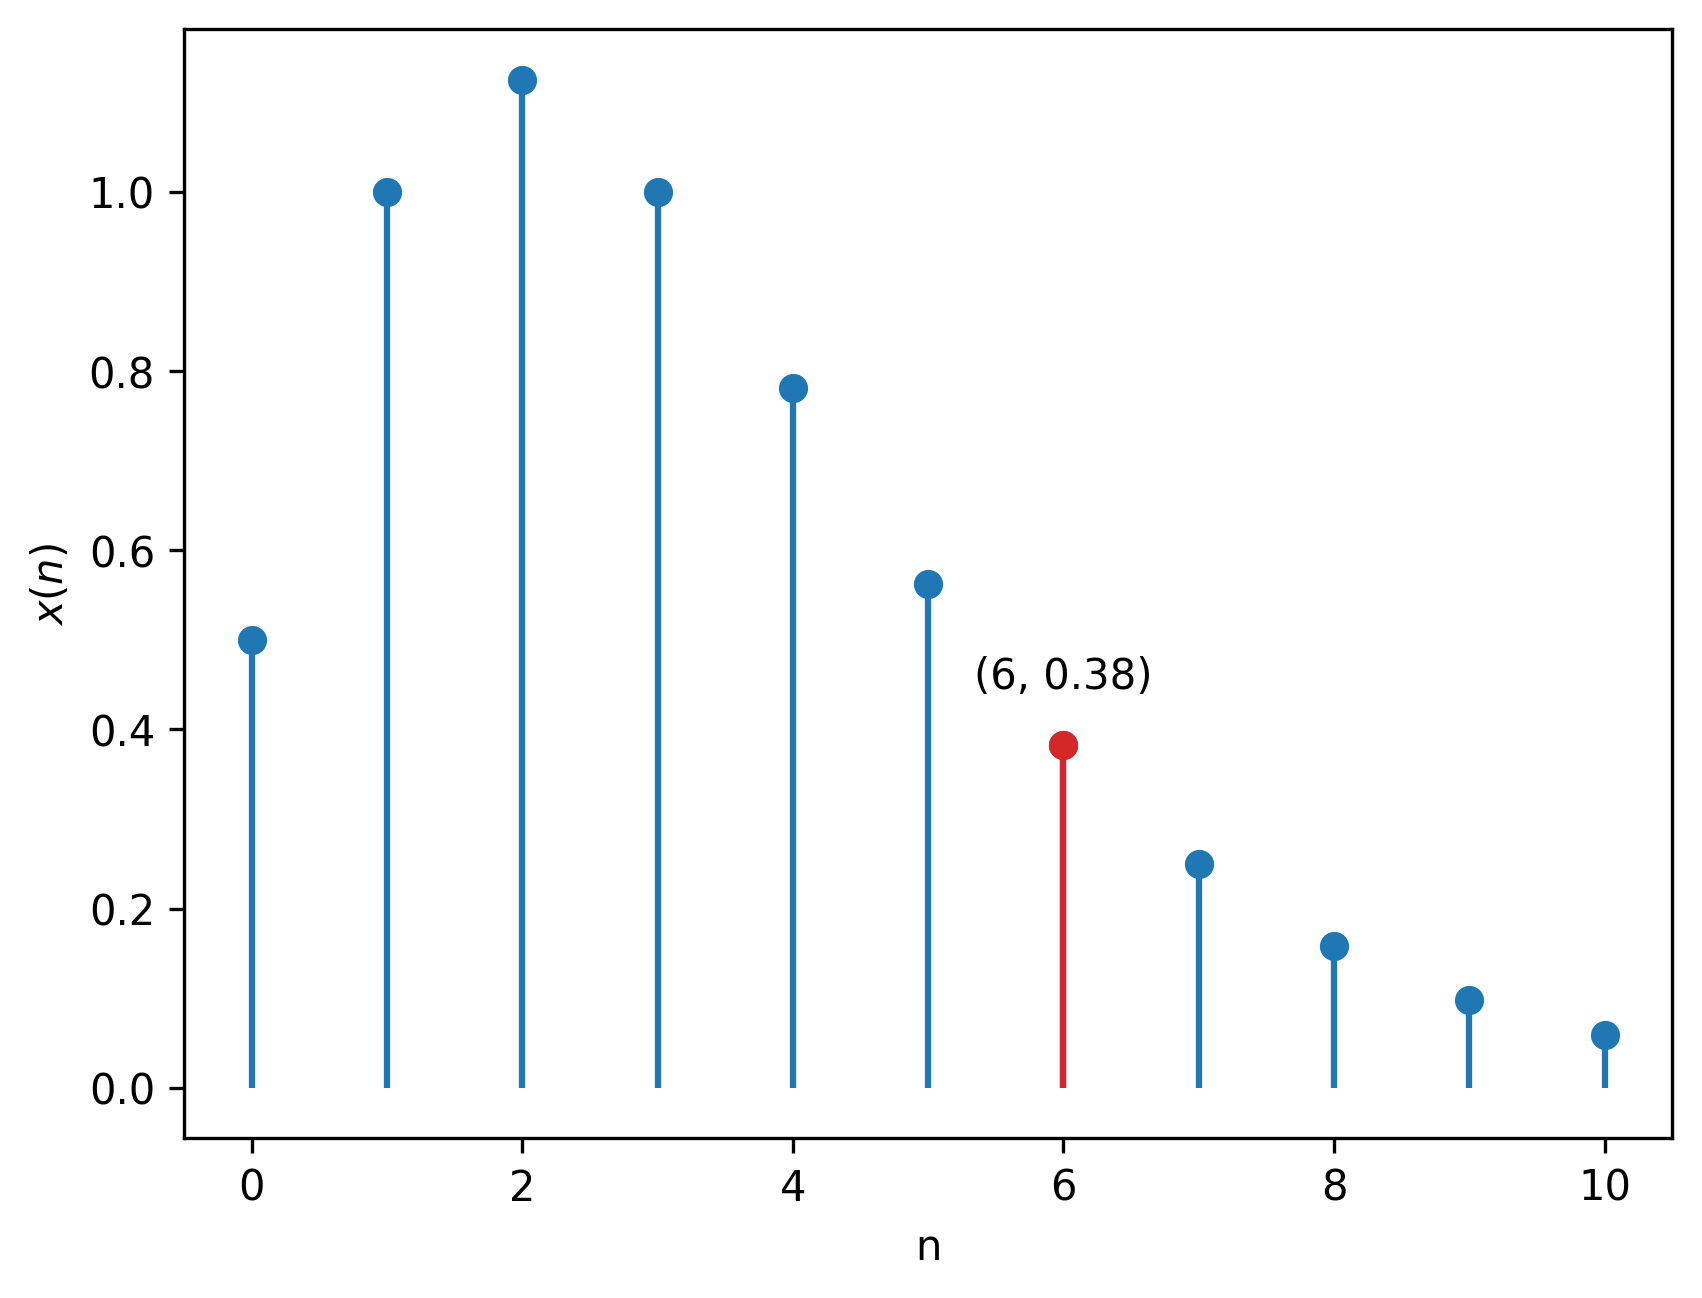
\includegraphics[width=\columnwidth]{ncert-maths/11/9/1/11.9.1.8/figs/plot.png}
    \caption{Stem plot of $x(n)$}
    \label{fig:1}
\end{figure}

%\end{document}


\pagebreak
\item For the travelling harmonic wave
$y\brak {x, t} = 2.0 \cos 2\pi \brak{10t - 0.0080 x + 0.35}$ where $x$ and $y$ are in $cm$ and $t$ in $s$. Calculate the phase difference between oscillatory
motion of two points separated by a distance of 

\begin{enumerate} [label=(\alph*)]
    \item $4 m$
    \item $0.5 m$
    \item $\lambda/2$
    \item $3\lambda/4$
\end{enumerate}
\solution
\iffalse
\let\negmedspace\undefined
\let\negthickspace\undefined
\documentclass[journal,12pt,twocolumn]{IEEEtran}
\usepackage{cite}
\usepackage{amsmath,amssymb,amsfonts,amsthm}
\usepackage{algorithmic}
\usepackage{graphicx}
\usepackage{textcomp}
\usepackage{xcolor}
\usepackage{txfonts}
\usepackage{listings}
\usepackage{enumitem}
\usepackage{mathtools}
\usepackage{gensymb}
\usepackage{comment}
\usepackage[breaklinks=true]{hyperref}
\usepackage{tkz-euclide} 
\usepackage{listings}
\usepackage{gvv}                                        
\def\inputGnumericTable{}                                 
\usepackage[latin1]{inputenc}                               \usepackage{caption}
\usepackage{color}                                            
\usepackage{array}                                            
\usepackage{longtable}                                       
\usepackage{calc}                                             
\usepackage{multirow}                                         
\usepackage{hhline}                                           
\usepackage{ifthen}                                           
\usepackage{lscape}

\newtheorem{theorem}{Theorem}[section]
\newtheorem{problem}{Problem}
\newtheorem{proposition}{Proposition}[section]
\newtheorem{lemma}{Lemma}[section]
\newtheorem{corollary}[theorem]{Corollary}
\newtheorem{example}{Example}[section]
\newtheorem{definition}[problem]{Definition}
\newcommand{\BEQA}{\begin{eqnarray}}
\newcommand{\EEQA}{\end{eqnarray}}
\newcommand{\define}{\stackrel{\triangle}{=}}
\theoremstyle{remark}
\newtheorem{rem}{Remark}
\begin{document}

\bibliographystyle{IEEEtran}
\vspace{3cm}

\title{NCERT 11.15. Q10}
\author{EE23BTECH11010 - Venkatesh Bandawar$^{*}$% <-this % stops a space
}
\maketitle
\newpage
\bigskip

\renewcommand{\thefigure}{\arabic{figure}}
\renewcommand{\thetable}{\arabic{table}}

\bibliographystyle{IEEEtran}

\parindent 0px
\textbf{Question:} For the travelling harmonic wave
$y\brak {x, t} = 2.0 \cos 2\pi \brak{10t - 0.0080 x + 0.35}$ where $x$ and $y$ are in $cm$ and $t$ in $s$. Calculate the phase difference between oscillatory
motion of two points separated by a distance of 

\begin{enumerate} [label=(\alph*)]
    \item $4 m$
    \item $0.5 m$
    \item $\lambda/2$
    \item $3\lambda/4$
\end{enumerate}

\solution
\fi
\begin{table}[htbp] \small
\centering
\begin{tabular}{|c|c|c|}
	\hline
	\textbf{Symbol} & \textbf{Value} & \textbf{Description} \\[6pt]
	\hline
	$x(0)$ & $25$ & first term of AP \\[6pt]
	\hline
	$d$ & $-3$ & common difference \\[6pt]
	\hline
	$x(n)$ & $(25-3n)u(n)$ & $n$-th term of AP \\[6pt]
	\hline
	$y(n)$ & $116$ & sum of terms \\[6pt]
	\hline 
\end{tabular}

\caption{Given \, parameters list}
\label{tab:11.15.10.1}
\end{table}
\begin{align}
    \brak{\Delta \theta} &= \brak{ 2\pi f t - kx_1 + \phi}  - \brak{2\pi f t -kx_2 + \phi}\\
    &= k\brak{x_2 - x_1} 
\end{align}

\begin{table}[htbp] 
\centering

      \begin{tabular}{|c|c|c|} 
      \hline
\textbf{Variable}& \textbf{Description}& \textbf{Value}\\\hline
         $x(n)$& $n^{th}$ term of sequence& $(2n+1)^2u(n)$\\\hline
          
    \end{tabular}


\caption{Phase \, differences}
\label{tab:11.15.10.2}
\end{table}

\begin{figure}[!h] 
\centering
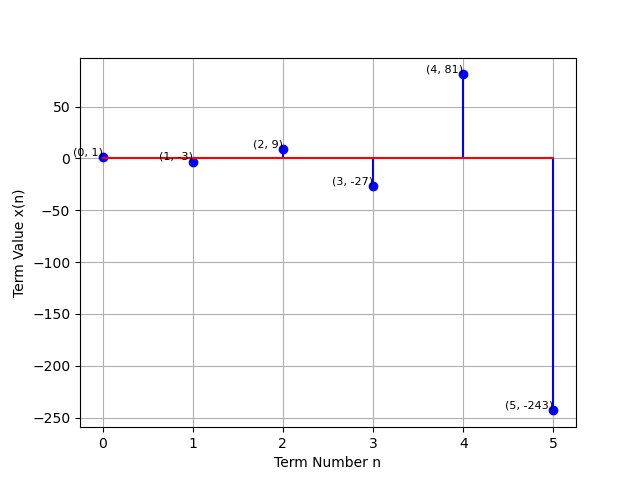
\includegraphics[width=\columnwidth]{ncert-physics/11/15/10/figs/graph1.png}
\captionsetup{justification=centering}
\caption{}
\label{fig:11.15.10.1}
\end{figure}

\begin{figure}[!h] 
\centering
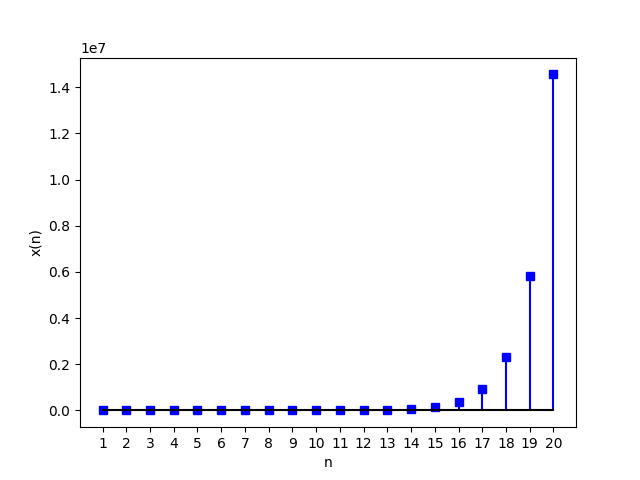
\includegraphics[width=\columnwidth]{ncert-physics/11/15/10/figs/graph2.png}
\captionsetup{justification=centering}
\caption{}
\label{fig:11.15.10.2}
\end{figure}

\begin{figure}[!h] 
\centering
\includegraphics[width=\columnwidth]{ncert-physics/11/15/10/figs/graph3.png}
\captionsetup{justification=centering}
\caption{}
\label{fig:11.15.10.3}
\end{figure}

\begin{figure}[!h] 
\centering
\includegraphics[width=\columnwidth]{ncert-physics/11/15/10/figs/graph4.png}
\captionsetup{justification=centering}
\caption{}
\label{fig:11.15.10.4}
\end{figure}



\pagebreak

\item Given below are some functions of x and t to 
represent the displacement (transverse
or longitudinal) of an elastic wave. State which of these represents \brak i travelling
wave, \brak {ii} a stationary wave or \brak {iii} none at all: 
\begin{enumerate}
\item $y = 2\cos \brak{3x} \sin \brak{10t}$
\item $y=2\sqrt{x-vt}$
\item $y = 3\sin \brak{5x - 0.5t} + 4\cos \brak{5x - 0.5t}$
\item $y = \cos x \sin t + \cos 2x \sin 2t$
\end{enumerate}
\solution
\iffalse
\let\negmedspace\undefined
\let\negthickspace\undefined
\documentclass[journal,12pt,twocolumn]{IEEEtran}
\usepackage{cite}
\usepackage{amsmath,amssymb,amsfonts,amsthm}
\usepackage{algorithmic}
\usepackage{graphicx}
\usepackage{textcomp}
\usepackage{xcolor}
\usepackage{txfonts}
\usepackage{listings}
\usepackage{enumitem}
\usepackage{mathtools}
\usepackage{gensymb}
\usepackage{comment}
\usepackage[breaklinks=true]{hyperref}
\usepackage{tkz-euclide} 
\usepackage{listings}
\usepackage{gvv}                                        
\def\inputGnumericTable{}                                 
\usepackage[latin1]{inputenc}                                
\usepackage{color}                                            
\usepackage{array}                                            
\usepackage{longtable}                                       
\usepackage{calc}                                             
\usepackage{multirow}                                         
\usepackage{hhline}                                           
\usepackage{ifthen}                                           
\usepackage{lscape}
\newtheorem{theorem}{Theorem}[section]
\newtheorem{problem}{Problem}
\newtheorem{proposition}{Proposition}[section]
\newtheorem{lemma}{Lemma}[section]
\newtheorem{corollary}[theorem]{Corollary}
\newtheorem{example}{Example}[section]
\newtheorem{definition}[problem]{Definition}
\newcommand{\BEQA}{\begin{eqnarray}}
\newcommand{\EEQA}{\end{eqnarray}}
\newcommand{\define}{\stackrel{\triangle}{=}}
\theoremstyle{remark}
\newtheorem{rem}{Remark}
\begin{document}
\parindent 0px
\bibliographystyle{IEEEtran}
\title{ASSIGNMENT11.15\_13Q}
\author{EE22BTECH11219 - Sai Sujan Rada$^{}$% <-this % stops a space
}
\maketitle
\newpage
\bigskip
\section*{QUESTION}
Given below are some functions of x and t to 
represent the displacement (transverse
or longitudinal) of an elastic wave. State which of these represents \brak i travelling
wave, \brak {ii} a stationary wave or \brak {iii} none at all: \\
\begin{enumerate}
\item $y = 2\cos \brak{3x} \sin \brak{10t}$
\item $y=2\sqrt{x-vt}$
\item $y = 3\sin \brak{5x - 0.5t} + 4\cos \brak{5x - 0.5t}$
\item $y = \cos x \sin t + \cos 2x \sin 2t$
\end{enumerate}
\solution 
\fi

\begin{table}[htbp]
    \centering
    \def\arraystretch{1.5}
    \begin{tabular}{|p{4cm}|p{4cm}|}
    \hline
TRAVELLING WAVE  & STATIONARY WAVE \\ \hline
    $y \brak{x,t} =A \sin  \brak{kx \pm \omega t} $ & $y\brak{ x,t }=A\sin kx\cos \omega t $ \\   \hline
    \hline
PARAMETERS  & DEFINITION  \\  \hline
$A$    &  Amplitude  \\ \hline
 $\omega$  & Angular Velocity  \\  \hline
 $x$    & Position  \\  \hline
 $k$    & Wavenumber    \\  \hline 
    \end{tabular}
    \caption{Travelling wave $vs$ Stationary wave}
    \label{tab:table11.13.1}
\end{table}

Let us assume an equation:
\begin{align}
y=A(x)\cos \brak{\omega t+\phi\brak {x}}
\end{align}
\begin{table}[htbp]
    \centering
    \def\arraystretch{1.5}
    \begin{tabular}{|p{4cm}|p{4cm}|}
    \hline
STATIONARY WAVE CONDITION & TRAVELLING WAVE CONDITION \\ \hline
        \brak 1 $A(x)$ should be a function of position x, and it can be expressed as $A(x)=A_{0}cos(\omega t+\alpha)$ where $A_{0}$ is a constant, $k$ is the wavenumber, $x$ is the position and $\alpha$ is a phase constant. & 
        \brak 1 $A(x)$ should be a constant, and it can be expressed as $A(x)=A_{0}$ where $A_{0}$ is a constant number. \\ \hline

        \brak 2 $\phi (x)$ can be expressed as $\phi (x)=c$ where c is a constant. &
        \brak 2 $\phi (x)$ represents a linear expression in x, and it can be expressed as $\phi (x)=kx+\theta$ where k is the wavenumber and $\theta$ is the phaseconstant. \\ \hline
\end{tabular}
    \caption{Travelling wave $vs$ Stationary wave}
    \label{tab:table11.13.2}
\end{table}

\begin{figure}[h]
                        \centering
                        \includegraphics[width=\columnwidth]{ncert-physics/11/15/13/figs/a.png}
                        \caption{DIPLACEMENT $vs$ TIME-graph1}
                        \label{fig:11.13.1}
\end{figure}
\begin{figure}[h]
                            \centering
                            \includegraphics[width=\columnwidth]{ncert-physics/11/15/13/figs/b.png}
                            \caption{DIPLACEMENT $vs$ TIME-graph2}
                            \label{fig:11.13.2}
\end{figure}   
\begin{figure}[h]
                             \centering
                             \includegraphics[width=\columnwidth]{ncert-physics/11/15/13/figs/c.png}
                             \caption{DIPLACEMENT $vs$ TIME-graph3}
                             \label{fig:11.13.3}
\end{figure}
\begin{figure}[h]
                            \centering
                            \includegraphics[width=\columnwidth]{ncert-physics/11/15/13/figs/d.png}
                            \caption{DIPLACEMENT $vs$ TIME-graph4}
                            \label{fig:11.13.4}
\end{figure}
\figref{fig:11.13.1} and \figref{fig:11.13.3} are self explanatory for stationary and travelling waves.
\figref{fig:11.13.2} and \figref{fig:11.13.4} are neither stationary nor travelling waves. 


\pagebreak

\end{enumerate}
